% Q22 椭圆与点线关系矢量示意。椭圆按方程取轴长；T 仅作 t>2/3 的代表位置，图不按比例。
% Source equation: \frac{(y+1)^2}{16}+\frac{(x-1)^2}{12}=1.
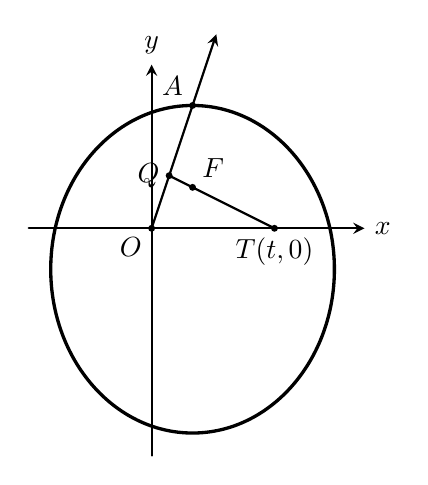
\begin{tikzpicture}[x=0.52cm,y=0.52cm,line cap=round,line join=round,>=stealth]
  \draw[->,thick] (-3.0,0)--(5.2,0) node[right] {$x$};
  \draw[->,thick] (0,-5.55)--(0,4.0) node[above] {$y$};

  % Ellipse center (1,-1), semiaxes 2sqrt(3) and 4.
  \draw[very thick] (1,-1) ellipse [x radius=3.4641,y radius=4];

  % A=(1,3) is the upper vertex and F=(1,1) the upper focus, as in the source figure.
  \coordinate (O) at (0,0);
  \coordinate (A) at (1,3);
  \coordinate (F) at (1,1);
  % A representative t=3 gives Q=(3/7,9/7); T is labeled parametrically.
  \coordinate (T) at (3,0);
  \coordinate (Q) at (0.4286,1.2857);

  \draw[thick,->] (O)--(1.58,4.74);
  \draw[thick] (T)--(Q);

  \fill (O) circle (1.25pt) node[below left] {$O$};
  \fill (A) circle (1.25pt) node[above left] {$A$};
  \fill (F) circle (1.25pt) node[above right] {$F$};
  \fill (T) circle (1.25pt) node[below] {$T(t,0)$};
  \fill (Q) circle (1.25pt) node[left] {$Q$};
\end{tikzpicture}
